\documentclass[10pt]{beamer}


\usetheme[progressbar=frametitle]{metropolis}
\usepackage{appendixnumberbeamer}

\usepackage{booktabs}
\usepackage[scale=2]{ccicons}

\usepackage{tabularx}
\usepackage{tikz}      % Diagrams

\usepackage[sfdefault,lf]{carlito}
\renewcommand*\oldstylenums[1]{{\carlitoOsF #1}}

\usepackage{pgfplots}
\usepgfplotslibrary{dateplot}
\usepackage[portuguese]{babel}
\usepackage{amsmath}
\usepackage{bm}

\usepackage{subcaption}

\usepackage{minted}

\usepackage{xspace}
\newcommand{\themename}{\textbf{\textsc{metropolis}}\xspace}

\title{
\includegraphics[scale=0.15]{figuras/logo-ipt.pdf} \hfill 
\includegraphics[scale=0.1]{figuras/usp-logo.pdf}\\Defesa de mestrado}
\subtitle{Uso de redes neurais convolucionais na recuperação de trecho de código-fonte}
% \date{\today}
\date{}
\author{Marcelo de Rezende Martins\\{\footnotesize sob orientação do Prof. Dr. Marco Aurélio Gerosa}}
\institute{Instituto de Pesquisas Tecnológicas do Estado de São Paulo - IPT}
% \titlegraphic{\hfill\includegraphics[height=1.5cm]{logo.pdf}}

\begin{document}

\maketitle



\section[Intro]{Introdução}


\begin{frame}[fragile]{Recuperação de trecho de código-fonte}

\begin{quote}
Recuperar um trecho de código-fonte relevante para atender a necessidade do usuário, descrita em linguagem natural.     
\end{quote}


\end{frame}



\section{Abordagem}

\begin{frame}{Agrupamento de vetores contínuos}
    \begin{figure}[h]
        \centering
        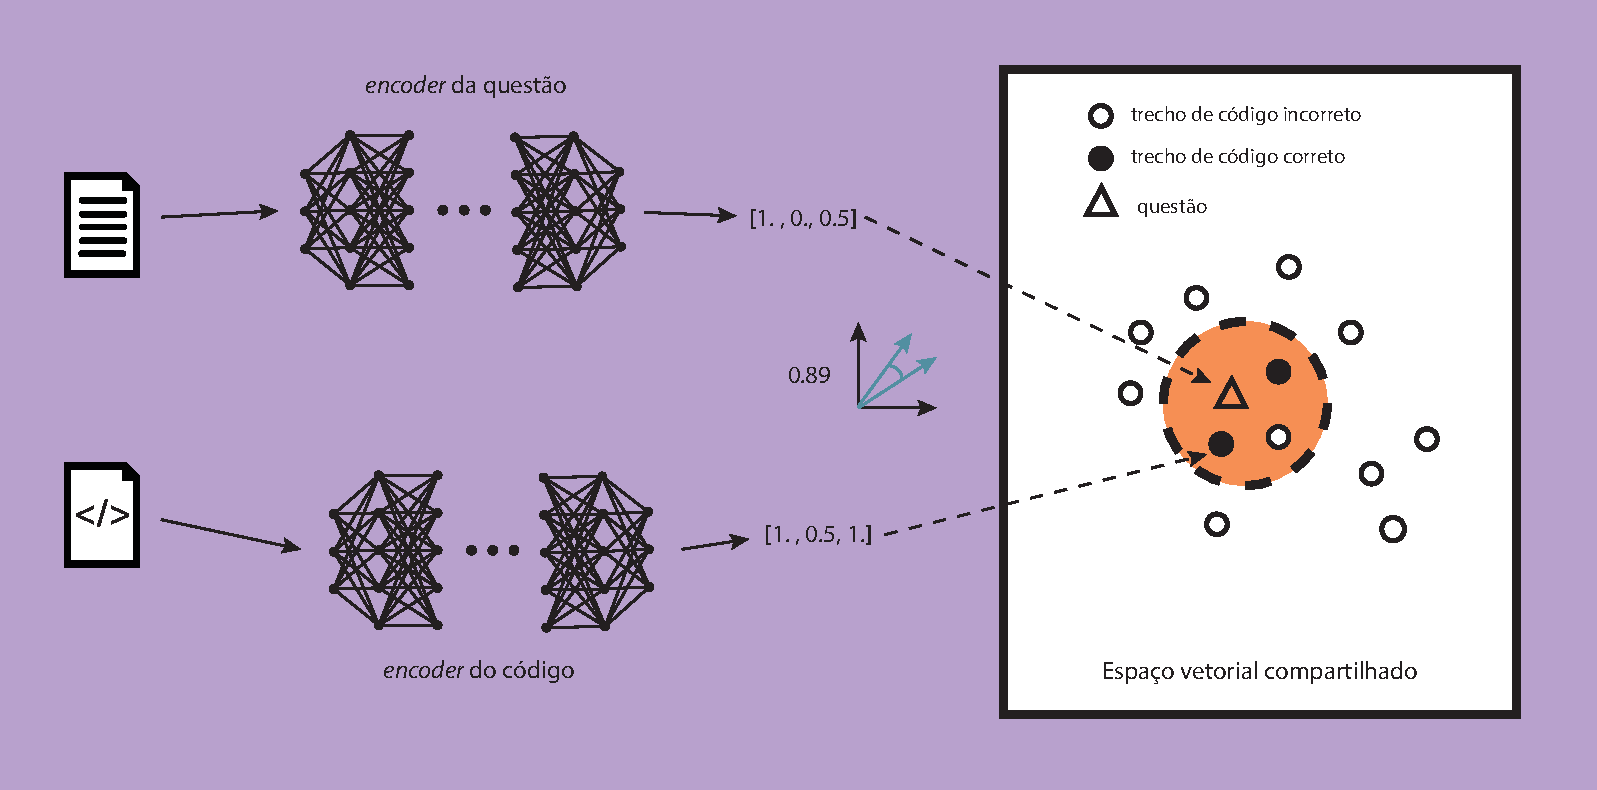
\includegraphics[width=1\linewidth]{figuras/joint_embedding.pdf}
        \caption{Ilustração da técnica de agrupamento de vetores contínuos na recuperação de trechos de código-fonte. }
        \label{fig:joint-embedding}
    \end{figure}
\end{frame}

\begin{frame}{Redes neurais convolucionais}
   \begin{figure}[h]
        \centering
        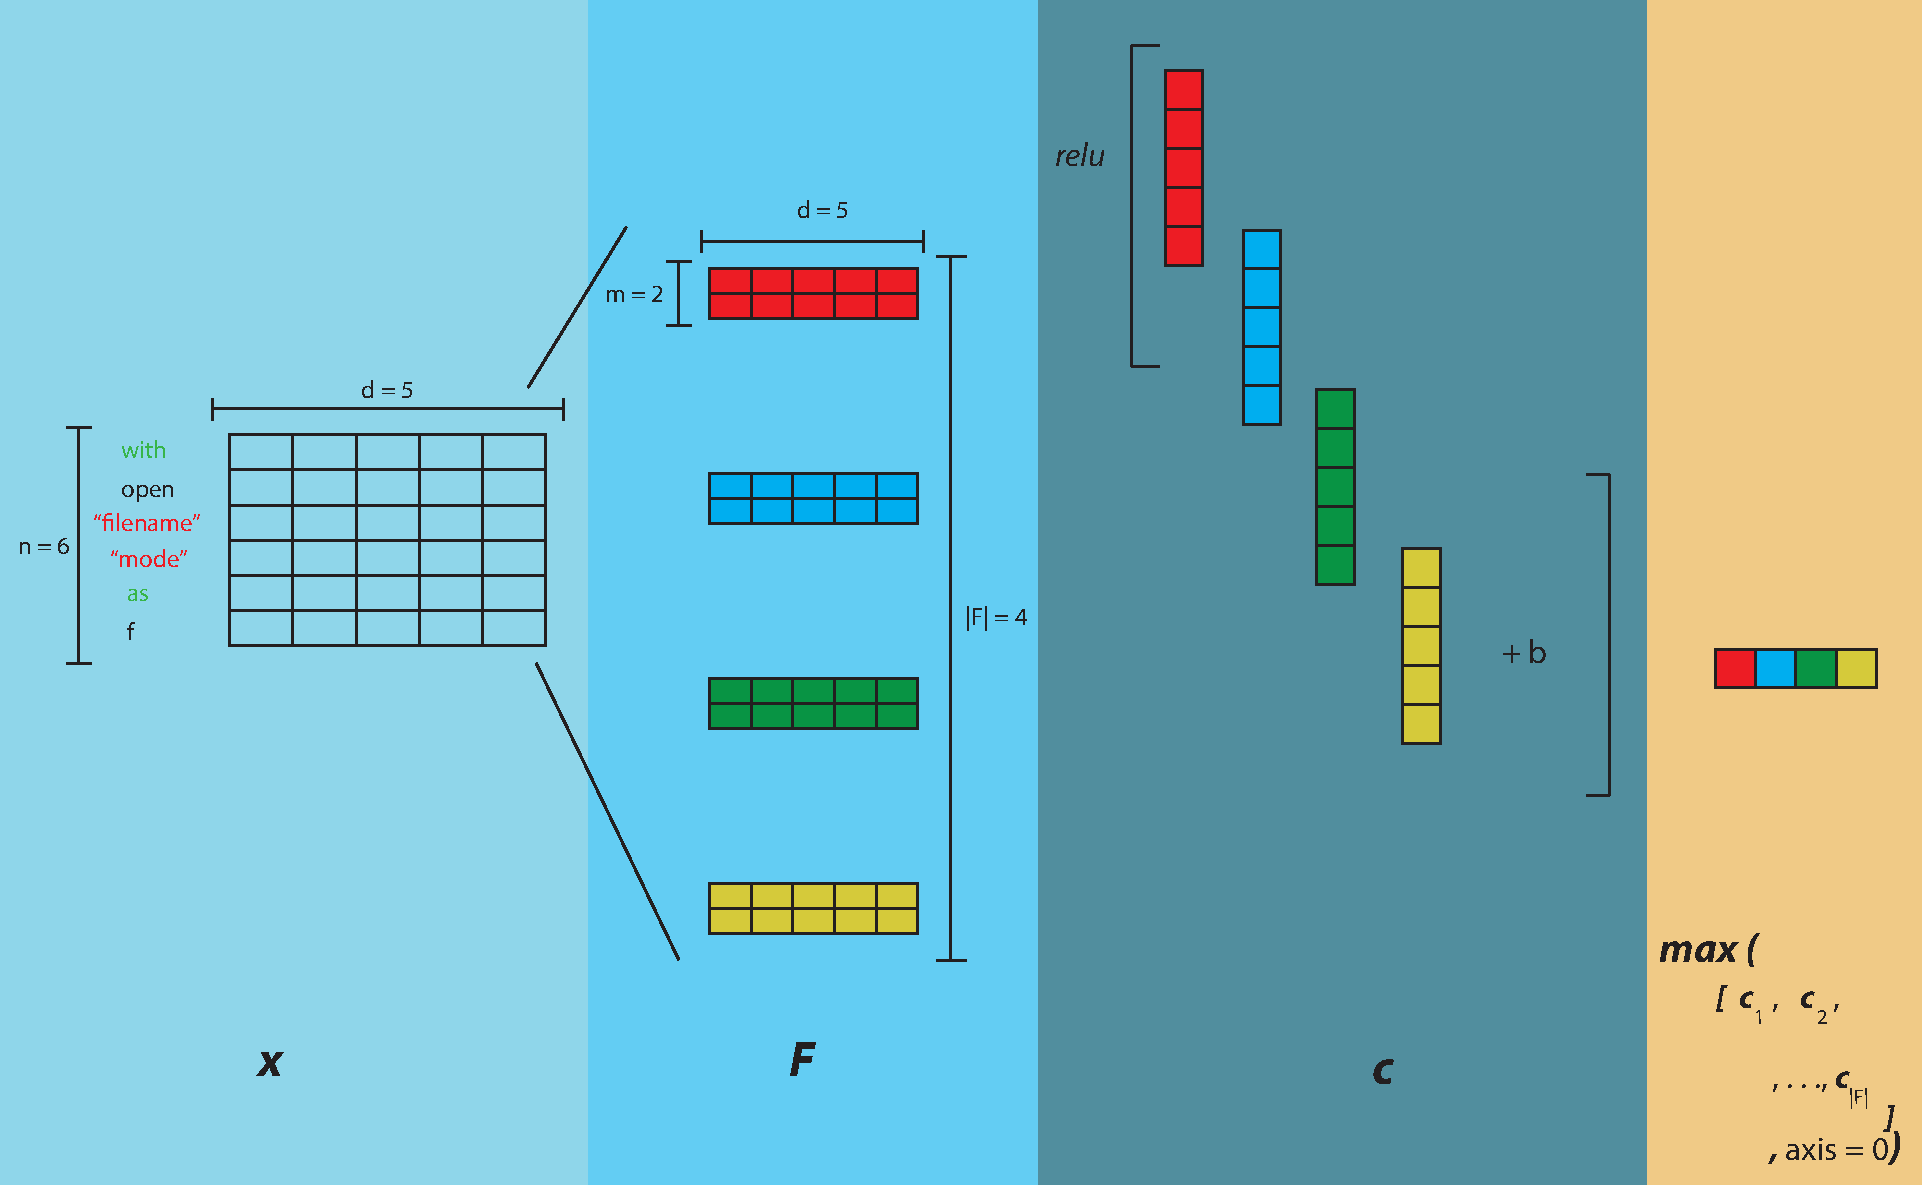
\includegraphics[width=1\linewidth]{figuras/cnn-steps-word-embedding-article.pdf}
        \caption{Ilustração das operações de convolução e \textit{max-pooling} realizada pela arquitetura proposta no trabalho. }
        \label{fig:convolution-steps}
    \end{figure}
\end{frame}






\section{Avaliação}

\begin{frame}{Amostra de treinamento e avaliação}
   \begin{table}[!b]
            %{\carlitoTLF % Use monospaced lining figures
        \begin{tabularx}{\textwidth}{Xrr}
            & \multicolumn{2}{c}{\textbf{Questão}}\\
            \toprule
          \textbf{Trecho de código-fonte} & \textbf{Python} & \textbf{SQL}  \\
          \toprule
          
            $N_{1}$: Apenas 1 trecho de código na descrição & $85.294$ & $75.637$ \\
            
            $N_{2}$: Mais de 1 trecho de código-fonte na descrição & $60.083$ & $41.826$ \\
            
            $N_{3}$: Trechos de códigos anotados manualmente & $2.169$ & $2.056$  \\
          \bottomrule
          \textbf{Total} & $\bm{147.546}$ & $\bm{119.519}$\\
          \bottomrule
        \end{tabularx}%}
        \caption{Sumário da amostra StaQC composta por questões e trechos de código-fonte extraídos do Stack Overflow.}
    \label{table:summary-training-data-yao-staqc}
        \end{table}
        \begin{tikzpicture}[overlay]
\draw[red,ultra thick,rounded corners] (7.85,2.32) rectangle (9.35,5.25);
\end{tikzpicture}
\end{frame}

\begin{frame}{Arquiteturas}
        \begin{figure}
          \begin{subfigure}[h]{0.45\textwidth}
            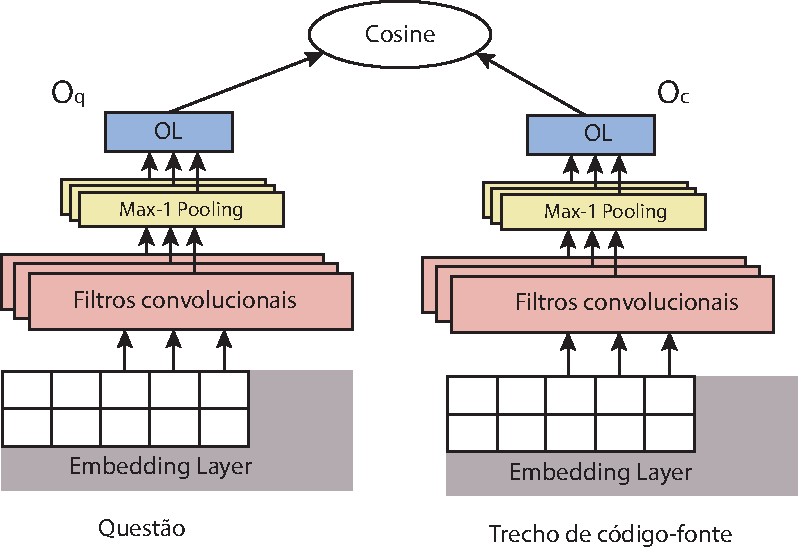
\includegraphics[width=\textwidth]{figuras/cnn-architecture-proposal.pdf}
            \caption{\textit{Nossa arquitetura}}
            \label{fig:our-architecture}
          \end{subfigure}
          \hspace{1em}%
          \begin{subfigure}[h]{0.45\textwidth}
            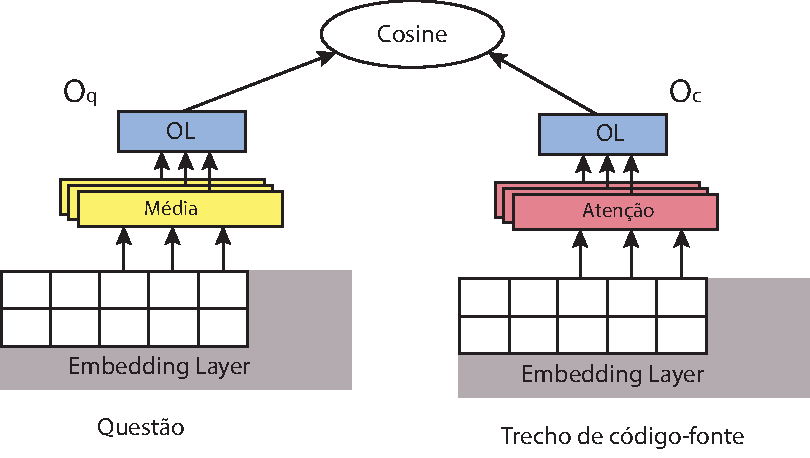
\includegraphics[width=\textwidth]{figuras/unif-architecture.pdf}
            \caption{Arquitetura SOTA}
            \label{fig:unif-architecture}
          \end{subfigure}
          
          \begin{subfigure}[h]{0.45\textwidth}
            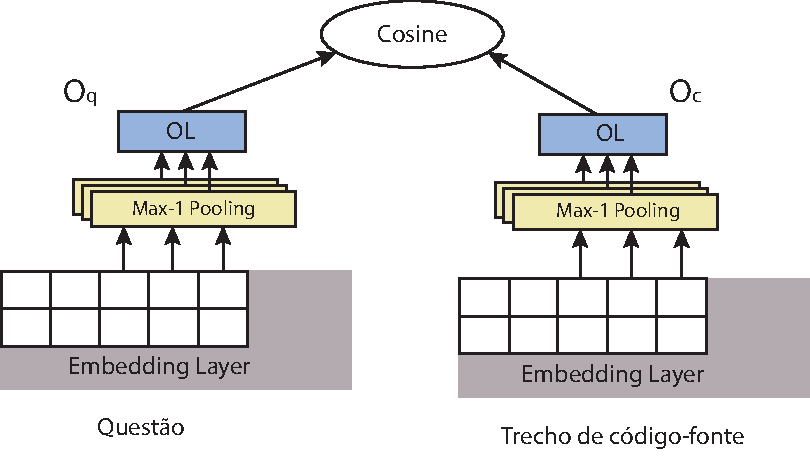
\includegraphics[width=\textwidth]{figuras/embedding-architecture.pdf}
            \caption{Arquitetura de referência}
            \label{fig:baseline-one-architecture}
          \end{subfigure}
        \end{figure}
\end{frame}



\section{Resultados}


\begin{frame}{Resultados}
\begin{table}[!b]
\footnotesize
  \begin{tabularx}{\textwidth}{XXX}
 \toprule
 \textbf{Modelos} & \textbf{MRR} & \textbf{TOP-1}\\
 \toprule
 Referência & $0.637$& $0.493 \pm 0.009$\\
 
 \bottomrule
 
 SOTA & $0.675 \pm 0.006$ & $0.539 \pm 0.009$\\
 
 \bottomrule
 
\textit{Nosso modelo} & $0.701 \pm 0.008$ & $0.577 \pm 0.015$\\
 
\bottomrule
\end{tabularx}
\caption{Resultados finais na amostra EVAL para o nosso modelo e os modelos de referência e SOTA. }
\label{table:resultados}
\end{table}
\end{frame}

\begin{frame}{Exemplos}
      \begin{figure}[h]
          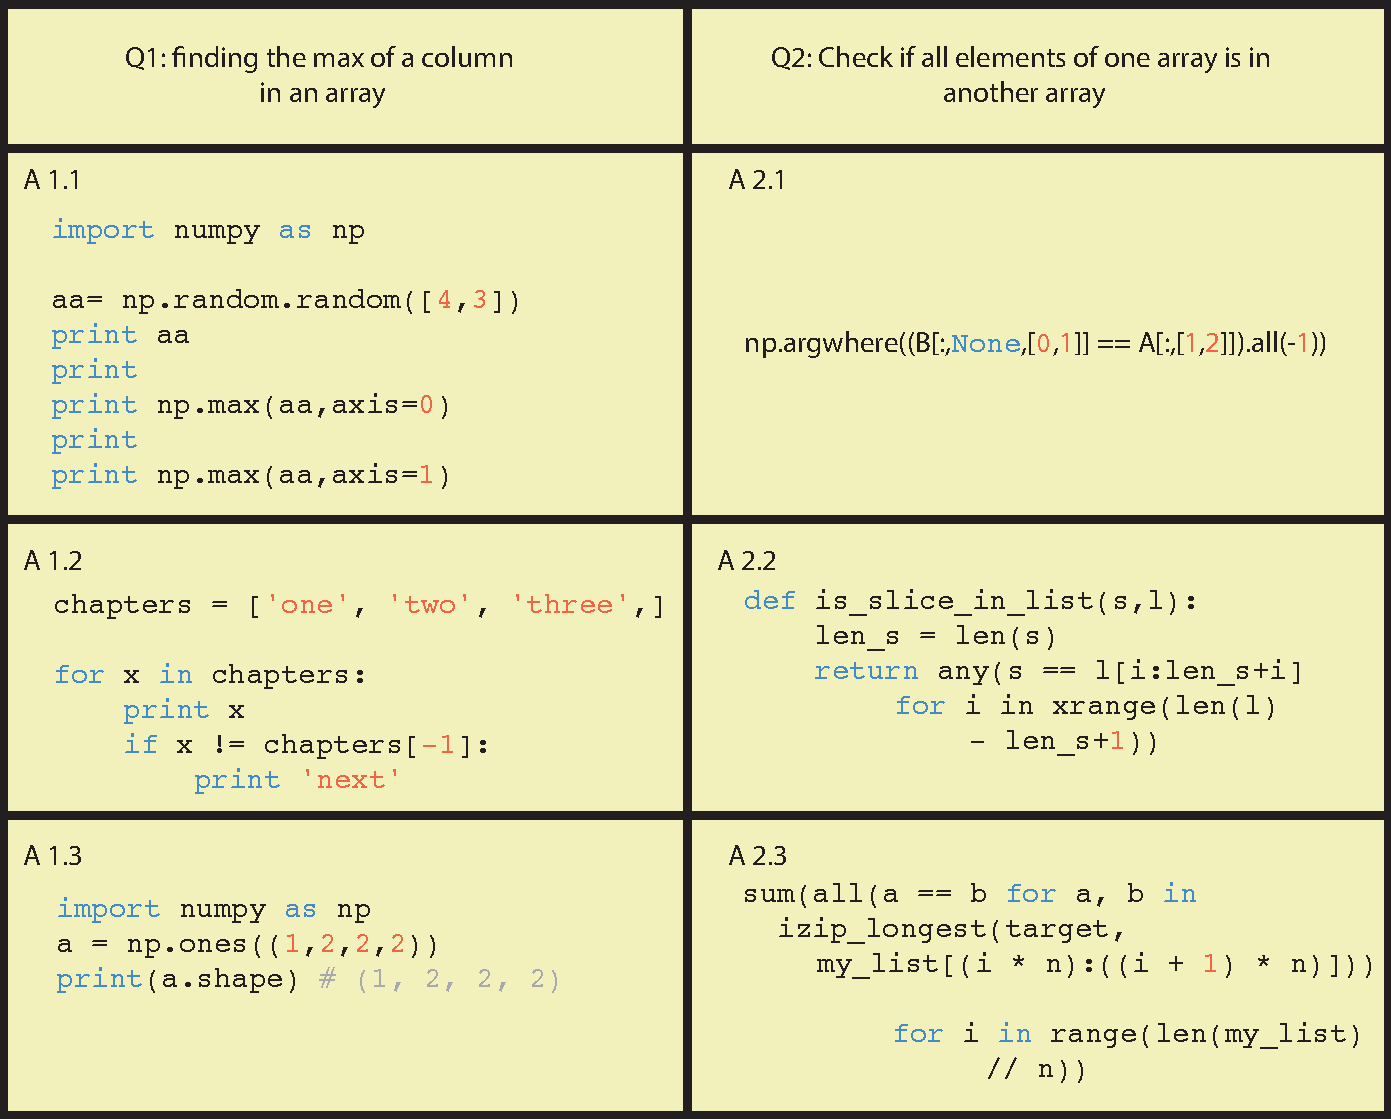
\includegraphics[width=0.75\textwidth]{figuras/concrete_examples.pdf}
          \caption{Exemplo de resposta correta selecionada pelo nosso modelo.}
          
          \label{fig:concrete-examples}
        \end{figure}
    \end{frame}
    


\section{Conclusão}

\begin{frame}{Conclusão}
        Nosso modelo obteve:
        \begin{itemize}
            \item Acurácia TOP-1 de 60\%, enquanto outros obtiveram 50\%;
            \item Top-3 de 78\%.
        \end{itemize}
\end{frame}
\begin{frame}{Futuras pesquisas}
        Futuras pesquisas:
        \begin{itemize}
            \item Avaliação de outras técnicas como \textit{transformers};
            \item Uso de treinamento não-supervisionado e transferência de aprendizagem;
            \item Encapsulamento dos modelos em uma ferramenta para avaliação e uso por usuários na prática.
        \end{itemize}
    \end{frame}


{\setbeamercolor{palette primary}{fg=black, bg=yellow}
\begin{frame}[standout]
  Perguntas?
\end{frame}
}

\appendix





\end{document}
